\hfill\small{16 Jan 2024}
\vspace{0.5em}
\hrule
\vspace{-0.5em}
\section{Lecture 4 --- Limit Cycles and Periodic Orbits}

Periodic orbits in the phase plane, which have a closed trajectory is usually 
called a perioidc orbit or closed orbit. An isolated perioidc orbit is called as a limit cycle.

For examples a harmonic oscillator has there is a continuum of cloed orbits as 
shown in the \autoref{fig:harmonic-oscillator}
, while in the case 
of Van der Pol oscillator, there is only one closed orbit i.e. a limit cycle as shown in
\autoref{fig:van-der-pol-oscillator}.

\begin{minipage}
    {0.5\textwidth}
    \begin{figure}[H]
        \centering
        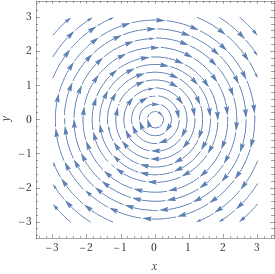
\includegraphics[width=0.9\textwidth]{figures/phaseportraits/osc.png}
        \caption{Harmonic Oscillator}
        \label{fig:harmonic-oscillator}
    \end{figure}
\end{minipage}
\begin{minipage}
    {0.5\textwidth}
    \begin{figure}[H]
        \centering
        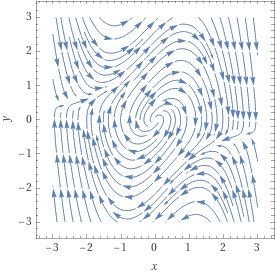
\includegraphics[width=0.9\textwidth]{figures/phaseportraits/van.png}
        \caption{Limit Cycle in Vander Pol Oscillator}
        \label{fig:van-der-pol-oscillator}
    \end{figure}
\end{minipage}

\subsection{Poincar\'e-Bendixson Theorem and Bendixson's Criterion}
Periodic orbits divide the plane into a region inside the orbit and a region outside it.
This allows us to obtains criteria for the existence of periodic orbits in a region of the plane.
The analysis of such a kind doesn;t extend to higher dimensions, as there is no concept of
inside and outside in higher dimensions. One such criteria is given by the Poincar\'e-Bendixson
theorem.

\begin{theorem}[Poincar\'e-Bendixson Theorem]
Let \(\dot{x} = f(x) , x \in \mathbb{R}^2\) and there exists a closed and bounded set
\(M \subset \mathbb{R}^2\) such that:
\begin{itemize}
    \item \(M\) contains no equillibrium points of \(\dot{x} = f(x)\)
    \item Every trajectory that starts in \(M\) remains in \(M\) for all \(t \geq 0\) 
\end{itemize} 
Then \(M\) contains a periodic orbit of \(\dot{x} = f(x)\).
\end{theorem}

\subsubsection*{Math Review:}
\[
    \Div f = \text{ divergence of vector field } f
\]
\[
    \Div f = \sum_{i=1}^{n} \frac{\partial f_i}{\partial x_i} \quad \text{where } f = (f_1, f_2, \dots, f_n)
\]
For a 2D vector field F we have:
\[
    \Div F = \frac{\partial f_1}{\partial x_1} + \frac{\partial f_2}{\partial x_2} \quad x \in \mathbb{R}^2
\]
If there are no sources or sinks in a region (which are equillibrium points in context 
of dynamical systems), then the divergence of the vector field is zero.

\begin{theorem}[Divergence and Green's Theorem]
    THe divergence theorem states that the volume integral of the divergence of a vector field
    is equal to the surface integral of the vector field over the boundary of the volume. i.e.
    \[
        \iiint{V} \Div F dV = \iint_{S} F \cdot n dS
    \]
    where \(n\) is the outward normal to the surface \(S\).

   Green's theorem states that the line integral of a vector field over a closed curve is equal
    to the surface integral of the curl of the vector field over the region bounded by the curve.
    i.e.
    \[
        \oint_{C} F \cdot dr = \iint_{S} \curl F \cdot n dS
    \]
    \[
        \implies \iint_S \left( 
            \frac{\partial f_1}{\partial x_1} + \frac{\partial f_2}{\partial x_2}
         \right) dS = \oint f_2(x_1, x_2) dx_1 - f_1(x_1, x_2) dx_2
    \]
\end{theorem}

Thus, we can now state teh Bendixson's criterion as follows:
\begin{theorem}[Bendixson's Criterion]
    Let \(D\) be a simply connected region in \(\mathbb{R}^2\). Suppose 
    \(f\) is such that \(\Div f = \dfrac{\partial f_1}{\partial x_1} + \dfrac{\partial f_2}
    {\partial x_2}\) is not identically zero in \(D\), and doesn't change sign in \(D\).
    Then there are no periodic orbits of \(\dot{x} = f(x)\) entirely in \(D\).
\end{theorem}
\begin{proof}
    Proof by contradiction: Suppose there exists a perioidc orbit \(\gamma \) that in 
    entirly in \(D\), for any trajectory of \(\dot{x} = f(x) \quad x \in \mathbb{R} ^{2} \)
    
    \[
        \frac{\mathrm{d}x_2}{\mathrm{d}x_1} = \frac{f_2 (x)}{f_1 (x)} \implies 
         f_2 (x) \mathrm{d}x_2 - f_1 (x) \mathrm{d}x_1 = 0
    \]
    \[
        \implies \oint_{\gamma} f_2 (x) \mathrm{d}x_2 - f_1 (x) \mathrm{d}x_1 = 0
    \]

    By Green's theorem, we have:
    \[
        \iint_S \left( 
            \frac{\partial f_1}{\partial x_1} + \frac{\partial f_2}{\partial x_2}
         \right) = 0
    \]

    This contradictcs the fact the divergence of \(f\) is not identically zero in \(D\), thus
    volating our assumption. Hence Proved.
\end{proof}

\subsection{Index of a curve}
\begin{definition}[Index of a curve]
    For a sufficiently smooth vector field \(f: \mathbb{R} ^{2} \to \mathbb{R} ^{2} \) and a 
    closed curve \(\gamma \) not passing through any equillibrium points of \(\dot{x} = f(x)\), the
    index of \(\gamma\) w.r.t.\ \(f\) is:
    \[
        I^f_\gamma = \frac{1}{2\pi} \oint_{\gamma} d\theta_f \qquad \theta = \tan^{-1} \left( 
            \frac{f_2}{f_1}
         \right)
    \]
\end{definition}
\vspace{1em}
There are certain properties of the index of a curve listed below:
\begin{property}[1]
    If we have two closed curves \(\gamma_1\) and \(\gamma_2\) such that \(\gamma_1\)
    can be continuously deformed into \(\gamma_2\) without passing through any equillibrium
    points then,
    \[
        I^f_{\gamma_1} = I^f_{\gamma_2}
    \]
\end{property}
\begin{property}[2]
    If \(\gamma \) doesn not enclose any equillibrium points, then
    \[
        I^f_{\gamma} = 0
    \] 
\end{property}
\begin{property}[3]
    \[
        I^f_\gamma = I^{-f}_\gamma 
    \]
    This can be intituitively understood as follows:
    \[
        \theta _f = \pi + \theta _{-f} \implies d\theta _f = - d\theta _{-f}
    \]
    Thus equating the line integral
\end{property}
\begin{property}[4]
    If \(\gamma \) is a closed orbit of \(\dot{x} = f(x)\) then
    \[
        I^f_\gamma = 1
    \]
\end{property}
\begin{property}[5]
    If \(\gamma \) encloses one equillibrium point \(x^*\), and \(x^{\star} \) is
    a hyperbolic equillibrium point, then:
    \[
        A = \left. \frac{\partial f}{\partial x} \right|_{x^{\star}} \implies 
        I^f_\gamma = I^{Ax}_\gamma 
    \] 
\end{property}

Using the above properties, we can now define the index of the equillibrium point.

\begin{definition}[Index of an equillibrium point]
\(I(x^{\star} _i)\) is the index of the equillibrium point \(x^{\star} _i\) of \(\dot{x} = f(x)\)
where \(I(x^{\star} _i)\) is the index of any closed curve \(\gamma \) enclosing only
\(x^{\star} _i\) and no other equillibrium points.  
\end{definition}
\begin{lemma}
    Index of a node, focus or a center is \(1\), while that of a saddle is \(-1\).
\end{lemma}
\begin{lemma}
    Index of a closed curve is the sum of the indices of the equillibrium points enclosed
    by the curve \(\gamma \)
\end{lemma}

Thus, we have the following corollary:

\begin{corollary}
    Inside any perioidc orbit \(\gamma \) there exists at least one equillibrium point. Suppose
    all the equillibrium points inside \(\gamma \) are hyperbolic. Let \(N\) be the number of
    nodes, foci and centers inside \(\gamma \) and \(S\) be the number of saddles inside \(\gamma \).
    then, the index of \(\gamma \) is:
    \[
        I^f_\gamma = N - S
    \] 
\end{corollary}